\section{Escalabilidade}
A escalabilidade é a capacidade de um sistema aumentar ou reduzir rapidamente a potência ou tamanho da infra-estrutura, de armazenamento ou de rede. Com a evolução dos requisitos e exigências dos recursos das aplicações, a escalabilidade da infra-estrutura de armazenamento proporciona um meio de adaptação às exigências dos recursos, otimizando os custos e melhorando a eficiência da equipa de \ac{IT}.

Escalabilidade Vertical (\textit{Scaling Up}) e Escalabilidade Horizontal (\textit{Scaling Out}) são métodos chave que as organizações utilizam para acrescentar capacidade às suas infra-estruturas. Para um utilizador final, estes dois conceitos podem parecer a mesma função. No entanto, cada um deles trata de necessidades específicas e resolve questões específicas de capacidade para a infra-estrutura do sistema de diferentes maneiras.

A escalabilidade vertical está a acrescentar mais recursos, como discos rígidos e memória, para aumentar a capacidade computacional dos servidores. Enquanto que a escalabilidade horizontal está a adicionar mais servidores à sua arquitetura para distribuir a carga de trabalho por mais máquinas.

\begin{figure}[H]
\center
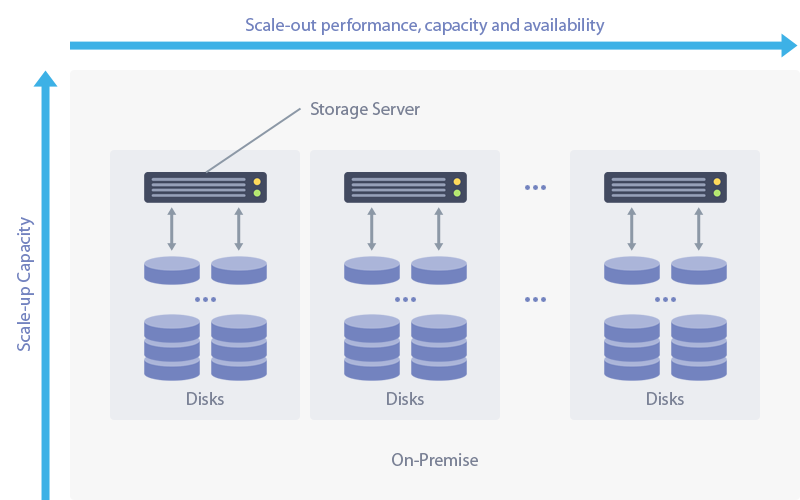
\includegraphics[width=12cm]{scaleup_out.png}
\caption{Escalabilidade Horizontal e Vertical}
\end{figure}

\section{Escalabilidade Horizontal (\textit{Scaling Out})}
A infra-estrutura da escalabilidade horizontal substitui o hardware pela funcionalidade, desempenho e capacidade de armazenamento. Esta escalabilidade resolve algumas das limitações da infra-estrutura, uma vez que é geralmente mais eficiente e eficaz. Além disso, a escalabilidade utilizando a nuvem (cloud) assegura que não terá de comprar novo hardware sempre que quiser atualizar o seu sistema.

\subsection{Fatores de Mudança na Escalabilidade Horizontal}
\begin{itemize}
    \item Estratégia de escalabilidade de longo prazo: Os componentes podem ser acrescentados ou removidos, dependendo dos seus objetivos;
    \item Atualizações flexíveis: A escalabilidade evita as limitações da depreciação da tecnologia;
    \item Distribuição (\textit{Load Balancing}) do armazenamento.
\end{itemize}

\subsection{Vantagens da Escalabilidade Horizontal}
\begin{itemize}
    \item Tecnologias mais recentes de servidores;
    \item Adaptabilidade às mudanças da procura;
    \item Gestão de custos.
\end{itemize}

\subsection{Desvantagens da Escalabilidade Horizontal}
\begin{itemize}
    \item Espaço em rack limitado;
    \item Custos operacionais acrescidos;
    \item Custos iniciais mais elevados.
\end{itemize}

\section{Escalabilidade Vertical (\textit{Scaling Up})}
A Escalabilidade Vertical da infra-estrutura visa acrescentar recursos de apoio a uma aplicação para melhorar ou manter um desempenho amplo. Tanto os recursos virtuais como de hardware podem ser aumentados/melhorados. No contexto do hardware, pode ser tão simples como utilizar um disco rígido maior para aumentar a capacidade de armazenamento.
O aumento da infra-estrutura é viável até que os componentes individuais sejam impossíveis de aumentar, tornando isto uma solução a curto prazo.

\subsection{Fatores de Mudança na Escalabilidade Vertical}
\begin{itemize}
    \item Impacto no desempenho: Um bom indicador de quando aumentar a escala é quando as suas cargas de trabalho começam a atingir os limites de desempenho, resultando no aumento da latência e desempenho causados pela capacidade de \ac{I/O} e \ac{CPU};
    \item Quando a otimização do armazenamento não funciona: Sempre que a eficácia das soluções de otimização do desempenho e da capacidade diminui, é tempo de mudança na escalabilidade vertical.
\end{itemize}

\subsection{Vantagens da Escalabilidade Vertical}
\begin{itemize}
    \item Velocidade;
    \item Simplicidade;
    \item Relação custo-benefício;
    \item Consumo de energia limitado;
\end{itemize}

\subsection{Desvantagens da Escalabilidade Vertical}
\begin{itemize}
    \item Latência;
    \item Mão de obra e riscos;
    \item Equipamento antigo.
\end{itemize}